\documentclass{article}

% if you need to pass options to natbib, use, e.g.:
%     \PassOptionsToPackage{numbers, compress}{natbib}
% before loading neurips_2026

% The authors should use one of these tracks.
% Before accepting by the NeurIPS conference, select one of the options below.
% 0. "default" for submission
\usepackage[nonanonymous]{neurips_2026}
\usepackage{graphicx}
\usepackage{times}
\usepackage{array}
\usepackage{amsmath,amssymb}
\usepackage{hyperref}
\usepackage{subcaption}
% the "default" option is equal to the "main" option, which is used for the Main Track with double-blind reviewing.
% 1. "main" option is used for the Main Track
%  \usepackage[main]{neurips_2026}
% 2. "position" option is used for the Position Paper Track
%  \usepackage[position]{neurips_2026}
% 3. "eandd" option is used for the Evaluations & Datasets Track
 % \usepackage[eandd]{neurips_2026}
 % if you need to opt-in for a single-blind submission in the E&D track:
 %\usepackage[eandd, nonanonymous]{neurips_2026}
% 4. "creativeai" option is used for the Creative AI Track
%  \usepackage[creativeai]{neurips_2026}
% 5. "sglblindworkshop" option is used for the Workshop with single-blind reviewing
 % \usepackage[sglblindworkshop]{neurips_2026}
% 6. "dblblindworkshop" option is used for the Workshop with double-blind reviewing
%  \usepackage[dblblindworkshop]{neurips_2026}

% After being accepted, the authors should add "final" behind the track to compile a camera-ready version.
% 1. Main Track
 % \usepackage[main, final]{neurips_2026}
% 2. Position Paper Track
%  \usepackage[position, final]{neurips_2026}
% 3. Evaluations & Datasets Track
 % \usepackage[eandd, final]{neurips_2026}
% 4. Creative AI Track
%  \usepackage[creativeai, final]{neurips_2026}
% 5. Workshop with single-blind reviewing
%  \usepackage[sglblindworkshop, final]{neurips_2026}
% 6. Workshop with double-blind reviewing
%  \usepackage[dblblindworkshop, final]{neurips_2026}
% Note. For the workshop paper template, both \title{} and \workshoptitle{} are required, with the former indicating the paper title shown in the title and the latter indicating the workshop title displayed in the footnote.
% For workshops (5., 6.), the authors should add the name of the workshop, "\workshoptitle" command is used to set the workshop title.
% \workshoptitle{WORKSHOP TITLE}

% "preprint" option is used for arXiv or other preprint submissions
 % \usepackage[preprint]{neurips_2026}

% to avoid loading the natbib package, add option nonatbib:
%    \usepackage[nonatbib]{neurips_2026}

\usepackage[utf8]{inputenc} % allow utf-8 input
\usepackage[T1]{fontenc}    % use 8-bit T1 fonts
\usepackage{hyperref}       % hyperlinks
\usepackage{url}            % simple URL typesetting
\usepackage{booktabs}       % professional-quality tables
\usepackage{amsfonts}       % blackboard math symbols
\usepackage{nicefrac}       % compact symbols for 1/2, etc.
\usepackage{microtype}      % microtypography
\usepackage{xcolor}         % colors
% Note. For the workshop paper template, both \title{} and \workshoptitle{} are required, with the former indicating the paper title shown in the title and the latter indicating the workshop title displayed in the footnote. 
\title{PowerInfer: Fast Large Language Model Serving with a Consumer-grade GPU}
\nolinenumbers

% The \author macro works with any number of authors. There are two commands
% used to separate the names and addresses of multiple authors: \And and \AND.
%
% Using \And between authors leaves it to LaTeX to determine where to break the
% lines. Using \AND forces a line break at that point. So, if LaTeX puts 3 of 4
% authors names on the first line, and the last on the second line, try using
% \AND instead of \And before the third author name.



\author{%
  Cuong Dang\\  
  \texttt{cuong.dang@ucf.edu} \\
  \And
  Hai Nguyen \\  
  \texttt{hai.nguyen@ucf.edu} \\
  \And
  Joshua Lowe \\  
  \texttt{jo201760@ucf.edu} \\
  \And
  Lam Nguyen \\  
  \texttt{lam.nguyen@ucf.edu} \\
}


\begin{document}


\maketitle


\begin{abstract}
Large language model (LLM) inference is constrained by memory bandwidth and accelerator memory capacity.
\textbf{PowerInfer}~\cite{song2024powerinferfastlargelanguage} exploits \textbf{activation locality} in ReLU-based feed-forward networks (FFNs): a relatively small subset of neurons accounts for a large fraction of non-zero activations, enabling \textbf{GPU--CPU hybrid} execution that keeps ``hot'' neurons on GPU while computing ``cold'' neurons on CPU only when needed.
We study \textbf{ReluLLaMA} at \textbf{7B} and \textbf{13B} scales via a four-phase workflow: (1)~artifact setup (sparse/dense GGUFs, activation profiles, builds), (2)~activation distribution profiling, (3)~throughput benchmarking, and (4)~hot-neuron overlap across prompt categories.
Using shipped activation statistics (7B) and layer summaries (13B), we quantify heavy-tailed activation frequencies, 80/90/95\% coverage thresholds, and a U-shaped layer-wise Gini profile.
We benchmark generation throughput for PowerInfer and llama.cpp on an Apple M4 Max CPU and compare to a vLLM GPU baseline on Newton (standard Llama-2 SiLU checkpoints at matched parameter scale).
Finally, we measure how ``hot'' neuron sets vary across five prompt categories using PyTorch hooks; Jaccard overlaps are high ($\approx\!0.75$--$0.83$ at 7B; $\approx\!0.70$--$0.77$ at 13B) with structured layer-wise variation.
Overall, results support locality as a robust empirical property while highlighting deployment and evaluation pitfalls (hardware/model mismatches and configuration sensitivity). Code is available at https://github.com/viennh/CAP6614-PowerInfer.

\end{abstract}



\section{Introduction}
Decoder-only transformers dominate modern NLP, but \textbf{serving} them at low latency stresses GPU memory and bandwidth.
Even with quantization, larger checkpoints may not fit in consumer VRAM; naive layer-wise offloading reduces VRAM pressure but often shifts the bottleneck to \textbf{PCIe transfers} and \textbf{CPU compute}, leaving the GPU underutilized.

PowerInfer's key observation is \textbf{activation locality}: in ReLU-based FFNs, activations are highly skewed---many neurons are zero for a given token, and the frequency of non-zero activations across tokens is heavy-tailed.
This makes it feasible to keep a stable ``hot'' subset of weights on GPU and compute only predicted-active cold neurons on CPU.

\textbf{Contributions (empirical).} We do not modify PowerInfer; instead we validate and contextualize its assumptions on ReluLLaMA-7B and extend multiple analyses to ReluLLaMA-13B:
\begin{itemize}
  \item \textbf{Locality profiling:} per-layer skew (Gini), cumulative coverage (80/90/95\%), and ranked-frequency behavior (7B detailed; 13B summarized).
  \item \textbf{Throughput benchmarking:} end-to-end generation tokens/sec across PowerInfer, llama.cpp, and vLLM under clearly stated hardware and model checkpoints.
  \item \textbf{Input dependence:} cross-prompt hot-neuron overlap (Jaccard), universal vs category-specific neurons, and density trends by layer (7B and 13B).
\end{itemize}

\section{Related Work}
\textbf{Contextual / activation sparsity.} Activation sparsity and dynamic skipping arise in contextual sparsity methods, notably Deja~Vu~\cite{liu2023dejavucontextualsparsity}, and in serving systems that exploit structured sparsity. PowerInfer~\cite{song2024powerinferfastlargelanguage} couples offline neuron-frequency profiles with online predictors to skip FFN computation at inference.

\textbf{Efficient inference stacks.} vLLM optimizes dense GPU serving, building on PagedAttention~\cite{kwon2023efficientmemorymanagementlarge} and continuous batching. llama.cpp provides portable CPU/GPU inference for GGUF models. These differ from PowerInfer's neuron-level hybrid sparse design; we use them as baselines for dense CPU behavior and a GPU throughput reference.

\textbf{ReLU LLaMA variants.} ReluLLaMA modifies LLaMA-style FFNs to use ReLU so activations can be exactly zero---a prerequisite for neuron-level skipping. Standard Llama-2 uses SiLU; therefore our vLLM runs use \texttt{meta-llama/Llama-2-*-hf} checkpoints as same-scale dense GPU references, not identical activations.

\section{Methodology}
\subsection{PowerInfer: offline policy and online hybrid execution}
PowerInfer combines a \textbf{one-time offline} phase (profile activations on representative data, then \textbf{solve a placement policy} that maps \textbf{hot} neurons to the \textbf{GPU} and \textbf{cold} neurons to the \textbf{CPU}, subject to activation impact and memory limits) with an \textbf{online} phase (an \textbf{input-conditioned predictor} for which neurons to activate on each step, then \textbf{hybrid} execution: GPU for hot paths, CPU for cold).
The design avoids running the full dense FFN for every neuron on every step by keeping frequently used weights and activations \textbf{near the GPU} and only \textbf{materializing} the long tail when the predictor says it matters.
This matches the system described by Song et al.~\cite{song2024powerinferfastlargelanguage}; a follow-on line of work (PowerInfer-2) extends similar ideas to even more constrained devices~\cite{xue2024powerinfer2fastlargelanguage}. Our \textbf{evaluation} (Phases 2--4) characterizes shipped profiles, throughput, and input-dependent hot sets on top of that design.

\begin{figure}[htbp]
  \centering
  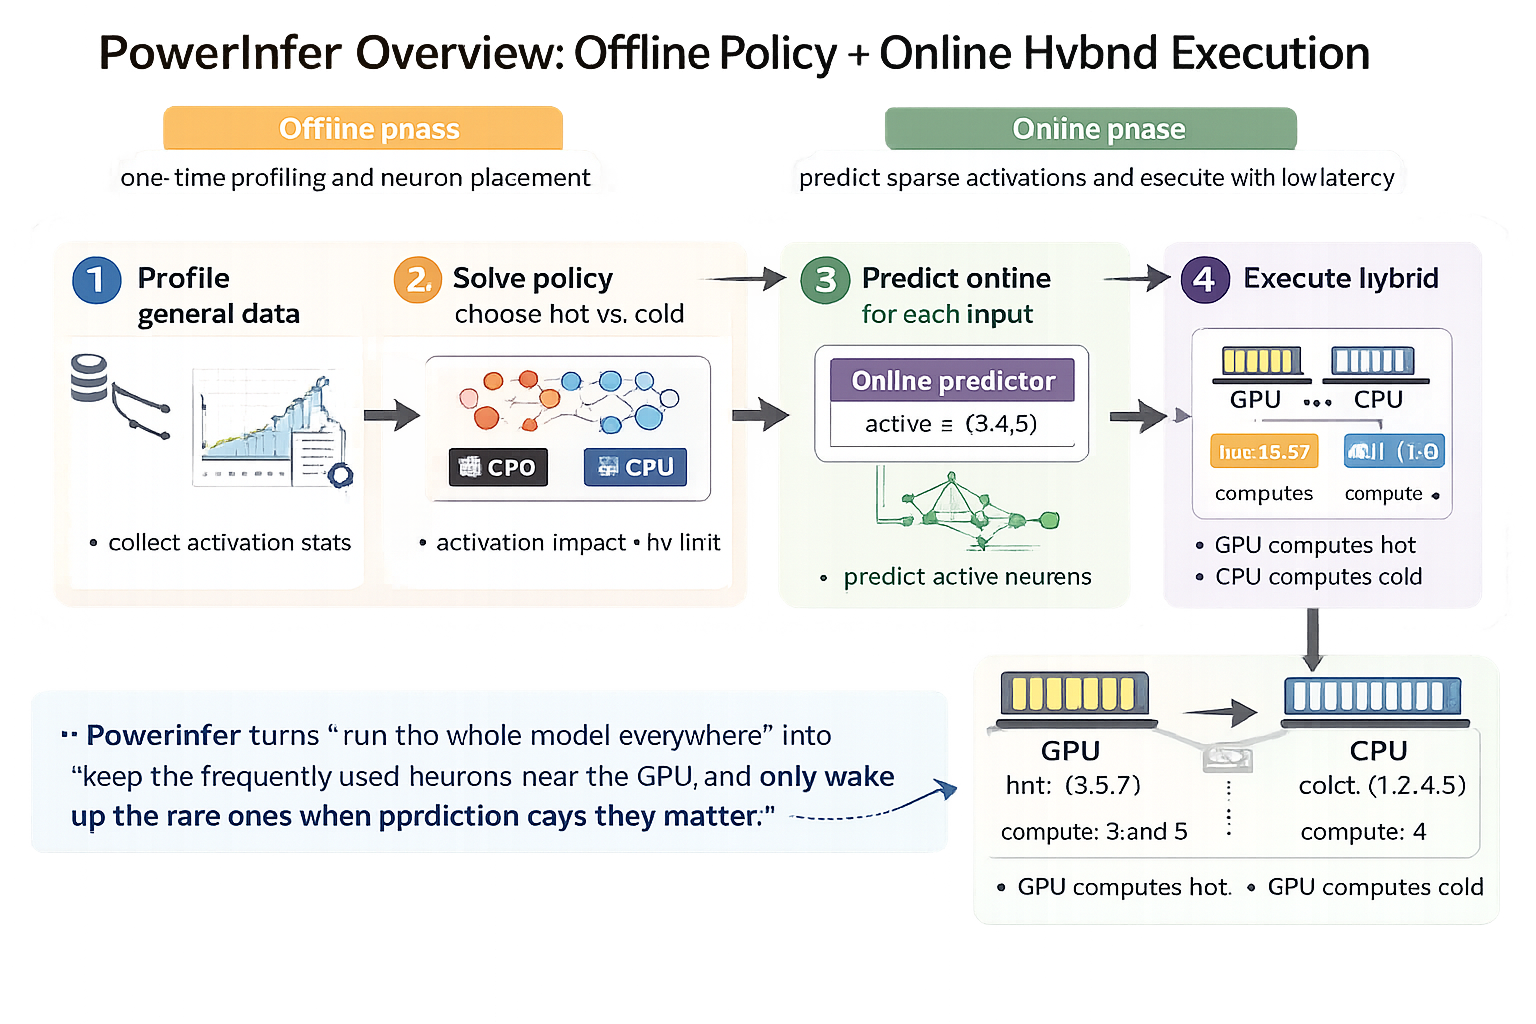
\includegraphics[width=0.95\linewidth]{figures/powerinfer-offline-policy-online-hybrid-exeution.png}
  \caption{\textbf{System view:} \textbf{offline} profiling and hot/cold \textbf{policy} (placement), then \textbf{online} prediction and \textbf{hybrid} GPU--CPU execution.}
  \label{fig:hybrid}
\end{figure}

\subsection{Four-phase experimental pipeline}
We organize experiments as a strict pipeline (same ordering as the course report):
\begin{enumerate}
  \item \textbf{Prerequisites \& artifacts:} sparse/dense GGUFs, \texttt{activation\_*.pt}, builds (PowerInfer and llama.cpp); optional HF checkpoints for Phase~4.
  \item \textbf{Activation profiling (Phase~2):} compute locality metrics from shipped activation statistics.
  \item \textbf{Throughput (Phase~3):} measure tokens/sec across engines for fixed prompts and output lengths.
  \item \textbf{Hot-neuron overlap (Phase~4):} instrument ReLU activations to compare hot sets across prompt categories.
\end{enumerate}
Phases 3 and 4 share an identical prompt suite to avoid confounding.

\begin{figure}[htbp]
  \centering
  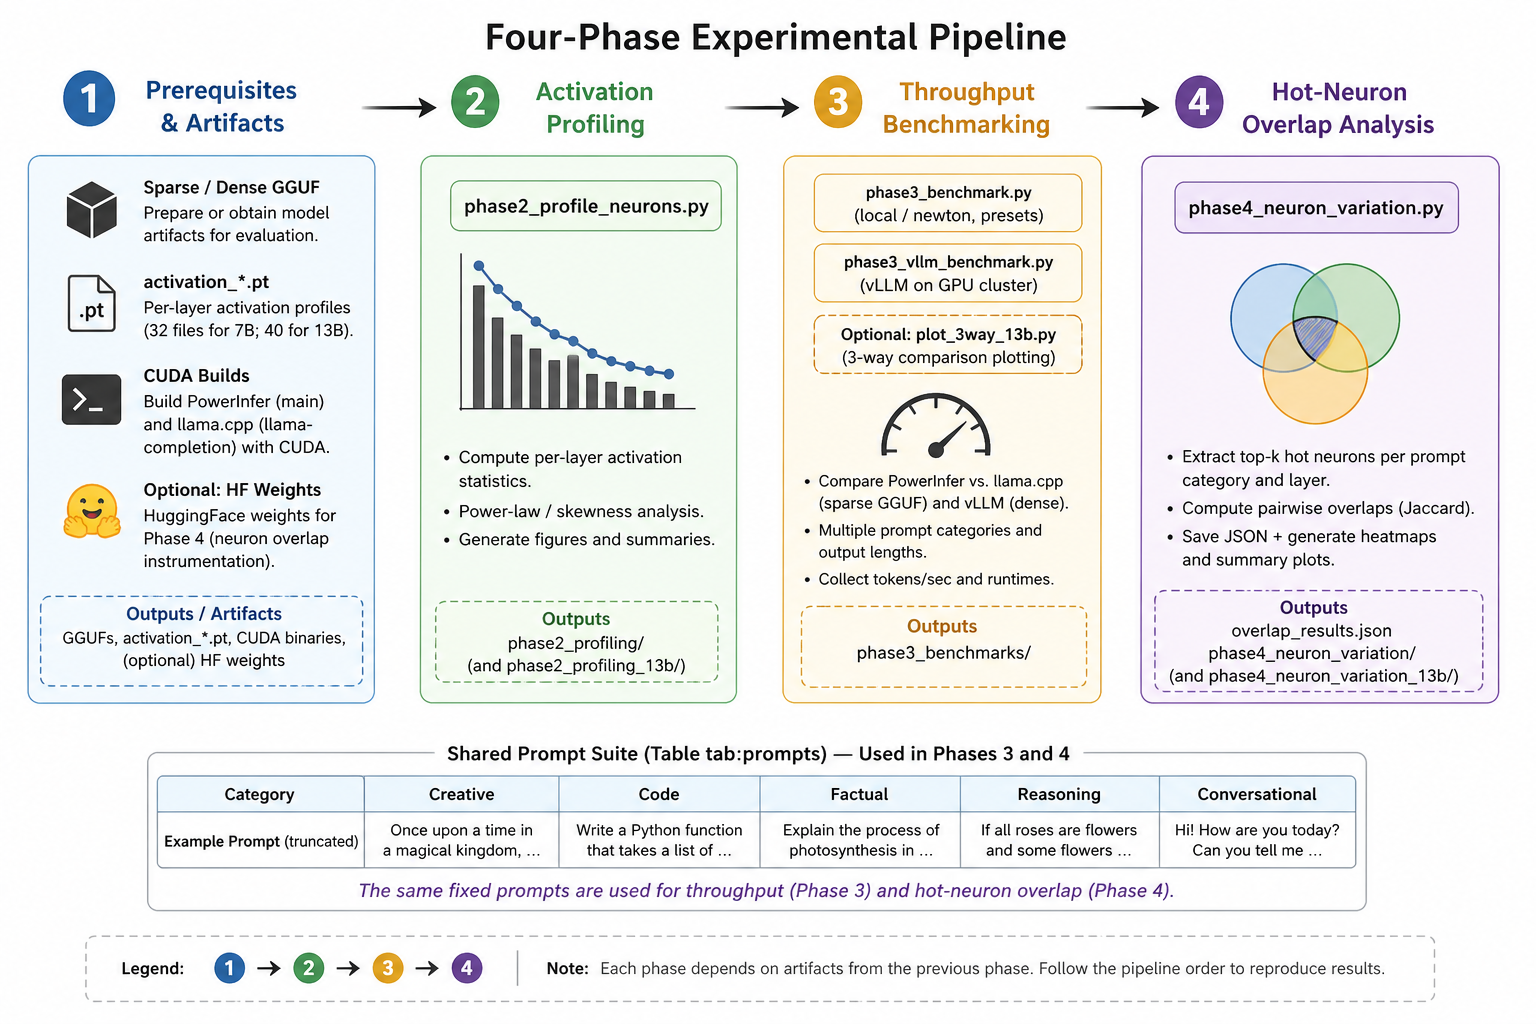
\includegraphics[width=0.95\linewidth]{figures/4-phase-experimental-benchmark-pipeline.png}
  \caption{\textit{Reproduction's workflow:} prerequisites, activation profiling, speed benchmarking, hot-neuron overlap, and the \textbf{shared prompt suite} (Phases 3--4).}
  \label{fig:pipeline}
\end{figure}

\subsection{Models and artifacts}
\textbf{ReluLLaMA-7B:} 32 transformer layers, hidden size 4096, FFN width 11008. We use PowerInfer GGUF (${\sim}$14GB FP16) plus shipped per-layer activation tensors \texttt{activation\_\{0..31\}.pt} (integer counts over a large profiling corpus, ${\sim}4\times 10^8$ activations per layer).

\textbf{ReluLLaMA-13B:} 40 layers, FFN width 13824. We use 13B PowerInfer artifacts (activation profiles and/or layer summaries for profiling summaries).

\subsection{PowerInfer system components}
\textbf{(1) Adaptive per-layer sparsity predictors.} PowerInfer uses an activation predictor to estimate which FFN neurons will be active for the current token. A fixed-size predictor for every layer can be prohibitively large at scale; PowerInfer sizes predictors per layer based on layer sparsity/skewness and tunes widths to keep perplexity near baseline.

\textbf{(2) Neuron-aware sparse operators.} Sparsity is dynamic and neuron-granular. Rather than relying on generic sparse libraries (which often require runtime format conversion), PowerInfer computes only rows/columns for predicted-active neurons using small neuron-index tables.

\textbf{(3) Placement solver and hybrid scheduling.} Offline placement is solved under VRAM and communication constraints to select GPU-resident ``hot'' neurons. Online, CPU and GPU execute operators from a DAG; synchronization is minimized and partial results are merged on GPU to keep the fast device on the critical path.

\subsection{Phase 2: activation distribution profiling}
From occurrence tensors we compute ranked frequencies, cumulative mass, neuron counts needed for 80/90/95\% coverage, and Gini coefficients per layer.

\subsection{Phase 3: throughput benchmarking}
We benchmark five prompt categories (Table~\ref{tab:prompts}) and generate $n \in \{32, 64, 128\}$ tokens with \texttt{--ignore-eos} for comparability.

\noindent\textbf{Local (7B):} PowerInfer vs llama.cpp on Apple M4 Max CPU (Accelerate BLAS).\\
\textbf{Newton (GPU reference):} vLLM FP16 on NVIDIA GPU nodes (CUDA 12.6).\\
\textbf{13B Newton snapshot:} llama.cpp dense and vLLM dense are reported; PowerInfer 13B generation rates in our snapshot are treated as misconfigured and are not used to support performance claims.

\subsection{Phase 4: input-dependent hot neurons}
We load HuggingFace ReluLLaMA weights and register forward hooks on FFN ReLU outputs. For each prompt category we generate 64 tokens and mark neurons as \textbf{hot} if ReLU output $>0$ for $\geq 10\%$ of generated positions. We report Jaccard similarity between categories, universal vs category-specific neurons, and layer-wise overlap trends.

\section{Experiments}
\begin{table}[htbp]
  \centering
  \small
  \caption{Prompt suite}
  \label{tab:prompts}
  \begin{tabular}{@{}p{0.15\linewidth}p{0.8\linewidth}@{}}
    \toprule
    Category & Prompt text \\
    \midrule
    Creative & Once upon a time in a magical kingdom, there lived a young princess who dreamed of exploring the world beyond the castle walls. \\
    Code & Write a Python function that takes a list of integers and returns the longest increasing subsequence using dynamic programming. \\
    Factual & Explain the process of photosynthesis in plants, including the light-dependent and light-independent reactions. \\
    Reasoning & If all roses are flowers and some flowers fade quickly, can we conclude that some roses fade quickly? Explain your reasoning step by step. \\
    Conversational & Hey, how are you doing today? I was thinking about learning a new programming language. Any suggestions? \\
    \bottomrule
  \end{tabular}
\end{table}

\subsection{Phase 2 (7B): locality and layer structure}
Activation frequency is strongly heavy-tailed but \textbf{layer dependent}. Early layers can be highly skewed (layer 0: Gini $\approx 0.533$; ${\sim}41.3\%$ neurons for 80\% coverage), while late-mid layers are more uniform (layer 24: Gini $\approx 0.182$; ${\sim}69.5\%$ for 80\%). Final layers regain skew (layer 31: Gini $\approx 0.522$). Nearly all neurons fire at least once globally, but frequencies span orders of magnitude---supporting a hot/cold split.

\begin{figure}[htbp]
  \centering
  \begin{subfigure}[t]{0.48\textwidth}
    \centering
    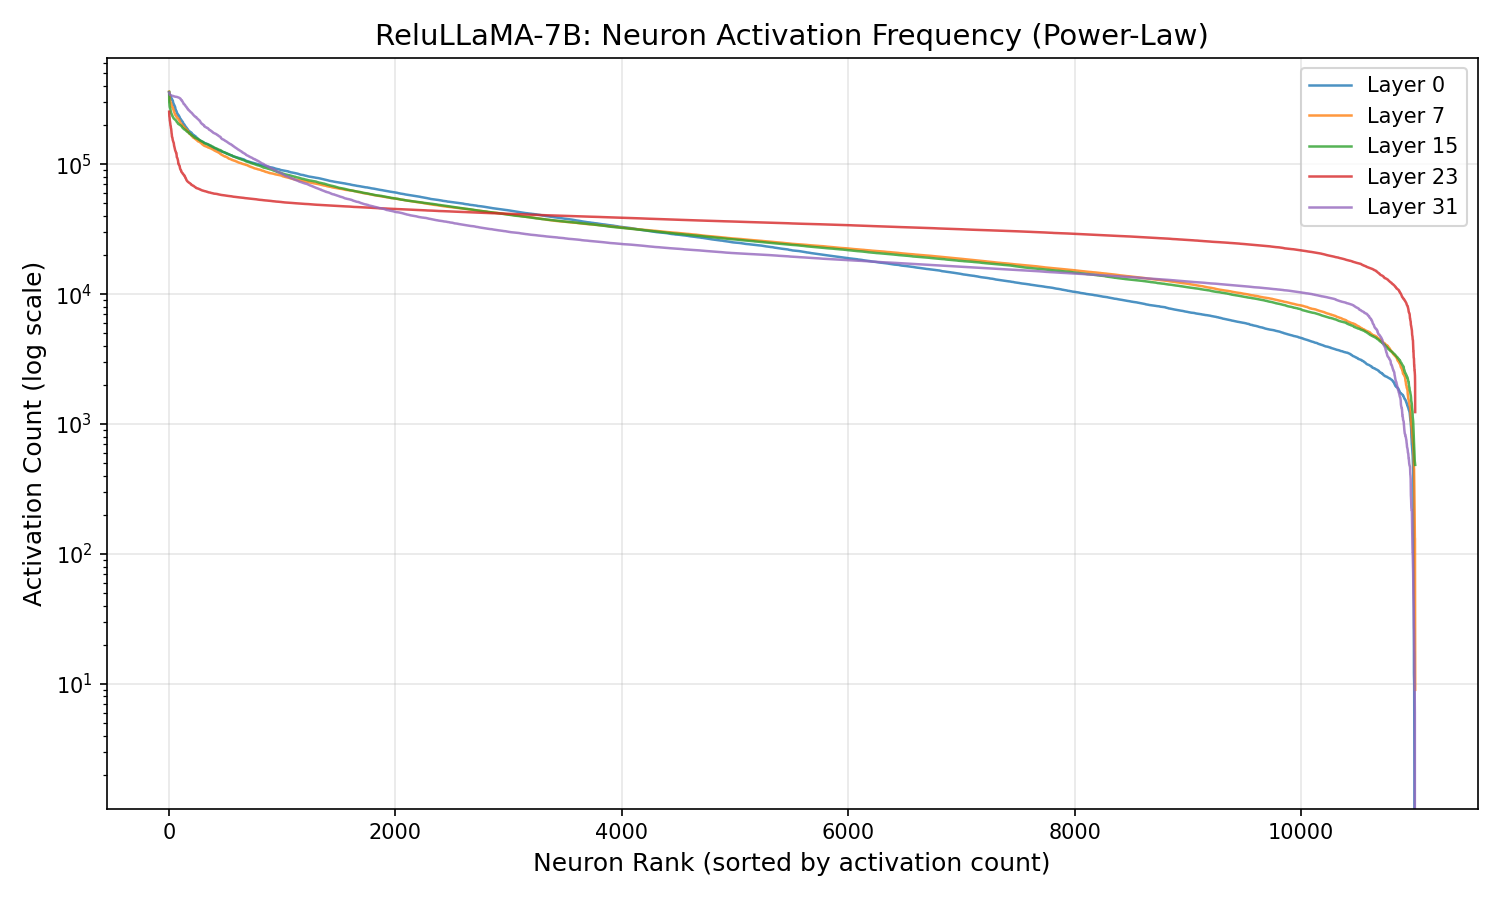
\includegraphics[width=\linewidth]{results/phase2_profiling/plot1_ranked_frequency.png}
    \caption{Ranked neuron activation frequencies (log scale), illustrating heavy tails.}
    \label{fig:p2-7b-rank}
  \end{subfigure}\hfill
  \begin{subfigure}[t]{0.48\textwidth}
    \centering
    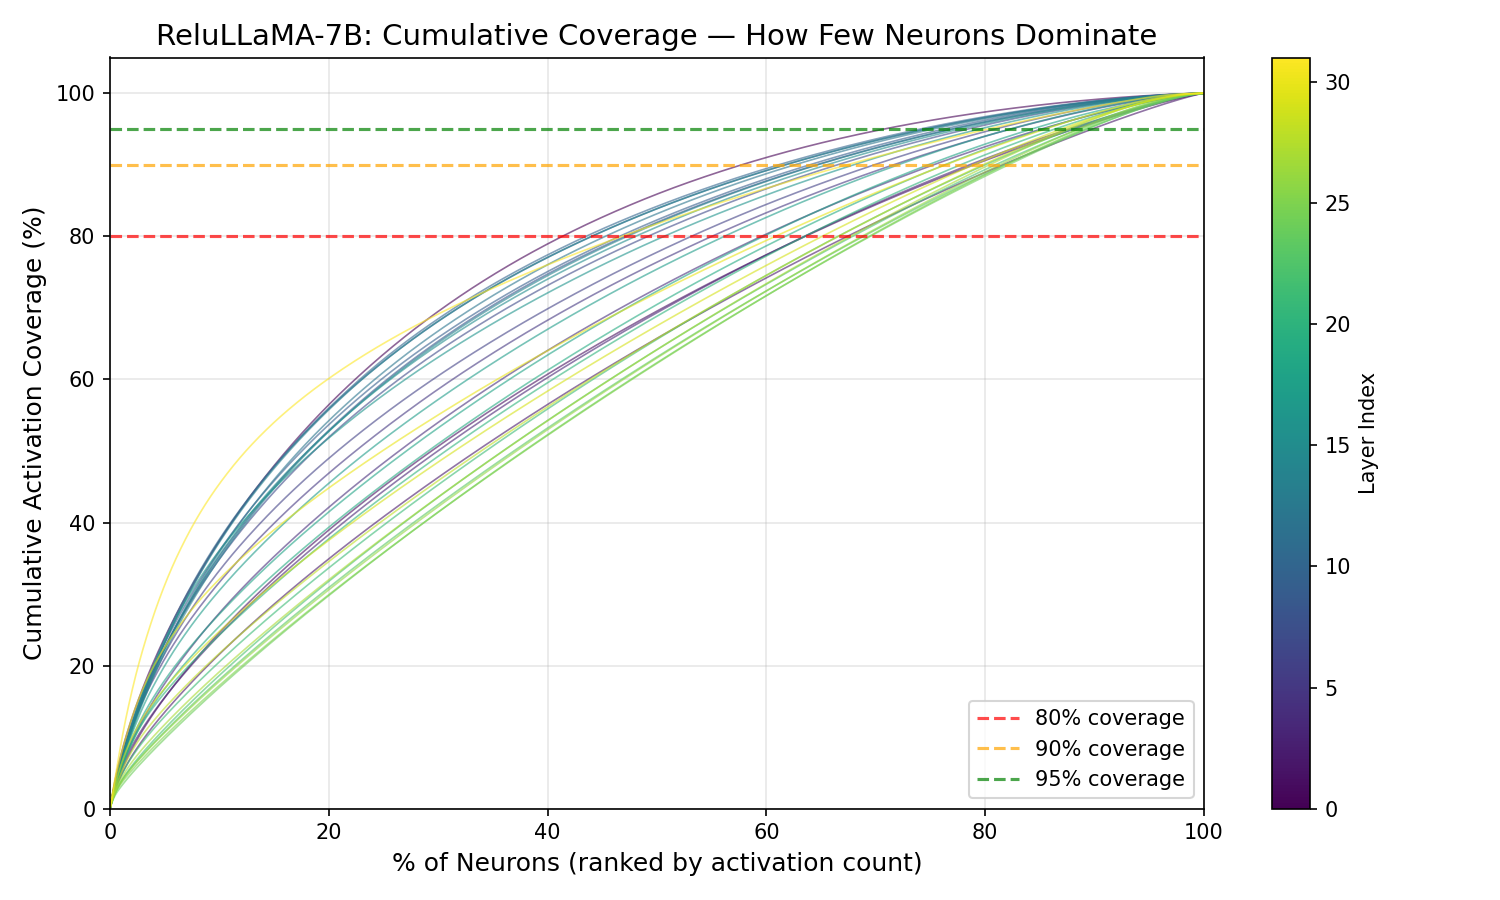
\includegraphics[width=\linewidth]{results/phase2_profiling/plot2_cumulative_coverage.png}
    \caption{Cumulative mass: fraction of total activations vs fraction of neurons (all layers).}
    \label{fig:p2-7b-cum}
  \end{subfigure}
  \par\medskip
  \hspace*{\fill}%
  \begin{subfigure}[t]{0.48\textwidth}
    \centering
    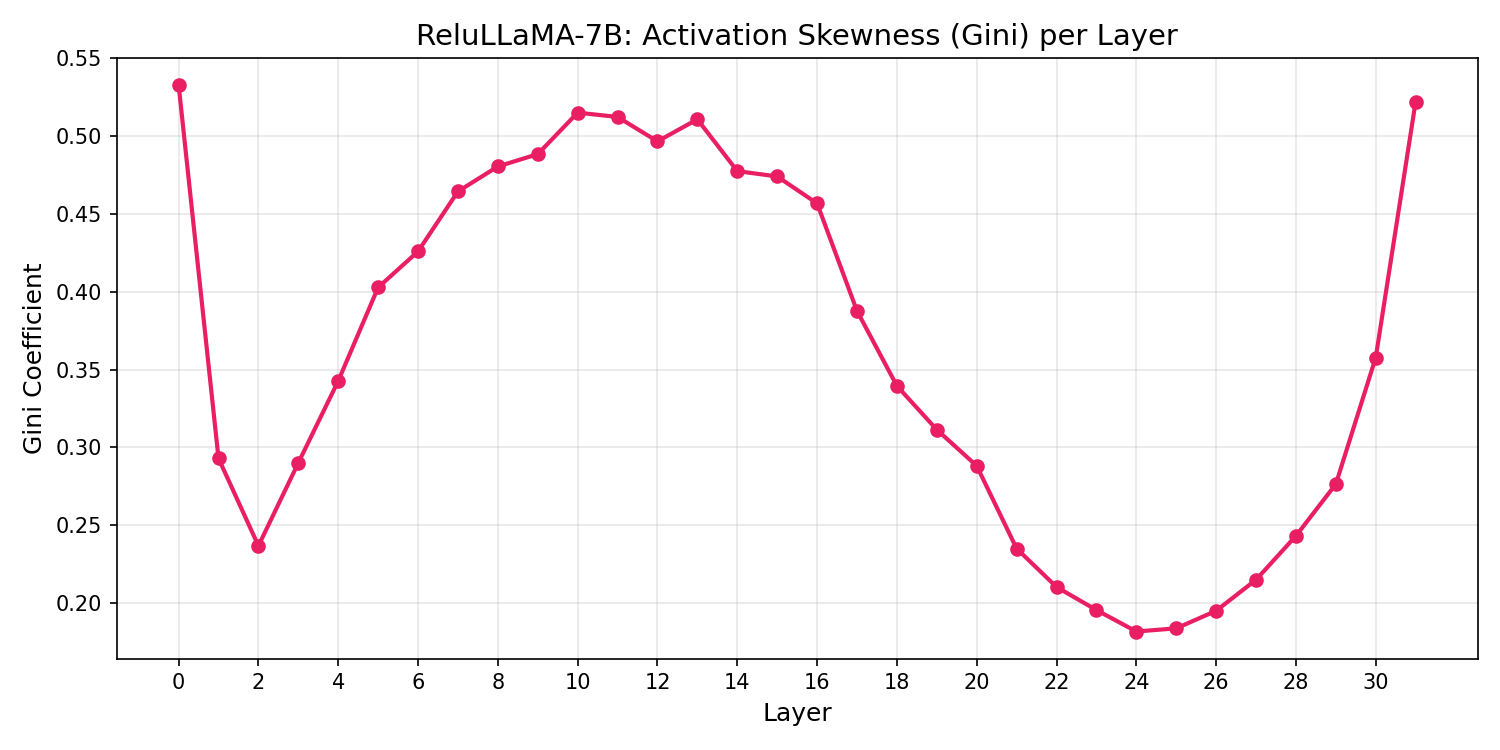
\includegraphics[width=\linewidth]{results/phase2_profiling/plot5_gini_by_layer.png}
    \caption{U-shaped Gini by layer (higher $=$ more unequal activation mass).}
    \label{fig:p2-7b-gini}
  \end{subfigure}%
  \hspace*{\fill}
  \caption{ReluLLaMA-7B Phase~2: activation locality (selected plots).}
  \label{fig:p2-7b-triple}
\end{figure}

\subsection{Phase 2 (13B): coverage snapshot}
From layer summaries, layer 0 is extremely skewed (Gini 0.660; 28.3\% neurons for 80\% coverage), while later layers can be more uniform (e.g., layer 20: 56.9\% for 80\%; layer 39: 56.6\%). The qualitative U-shape persists at larger width.


\begin{figure}[htbp]
  \centering
  \begin{subfigure}[t]{0.48\textwidth}
    \centering
    
\includegraphics[width=\linewidth]{results/phase2_profiling_13b/plot4_coverage_bars.png}
    \caption{Neurons needed for 80/90/95\% coverage per layer.}
    \label{fig:p2-13b-cov}
  \end{subfigure}\hfill
  \begin{subfigure}[t]{0.48\textwidth}
    \centering
    
\includegraphics[width=\linewidth]{results/phase2_profiling_13b/plot5_gini_by_layer.png}
    \caption{Gini vs layer (compare to 7B curve in Figure~\ref{fig:p2-7b-gini}).}
    \label{fig:p2-13b-gini}
  \end{subfigure}
  \caption{ReluLLaMA-13B Phase~2: activation locality summaries.}
  \label{fig:p2-13b-pair}
\end{figure}


\subsection{Phase 3 (7B): CPU throughput vs GPU ceiling}
On M4 Max CPU, llama.cpp is stable (${\sim}15$--$18$ tok/s generation) while PowerInfer is high-variance (0.77--20.59 tok/s) depending on prompt and length. PowerInfer matches/exceeds llama.cpp in some cases (e.g., code and conversational at $n{=}128$), but underperforms substantially in others (notably creative across lengths and several $n{=}64$ categories). On Newton GPU, vLLM reaches ${\sim}54$ tok/s after warm-up with $<1\%$ prompt variance.

\textbf{7B CPU throughput (Apple M4 Max)}
\begin{itemize}
  \item \textbf{$n{=}32$:} Creative 0.77 vs 3.18; Code 18.02 vs 16.08; Factual 16.98 vs 17.95; Reasoning 8.26 vs 9.92; Conversational 15.44 vs 17.70 (PowerInfer vs llama.cpp).
  \item \textbf{$n{=}64$:} Creative 0.94 vs 15.35; Code 6.47 vs 17.56; Factual 18.84 vs 17.86; Reasoning 5.37 vs 15.87; Conversational 4.95 vs 17.79.
  \item \textbf{$n{=}128$:} Creative 2.26 vs 15.77; Code 20.50 vs 17.57; Factual 7.99 vs 17.39; Reasoning 2.77 vs 16.71; Conversational 20.59 vs 17.95.
\end{itemize}

\begin{figure}[htbp]
  \centering
  \begin{subfigure}[t]{0.48\textwidth}
    \centering
    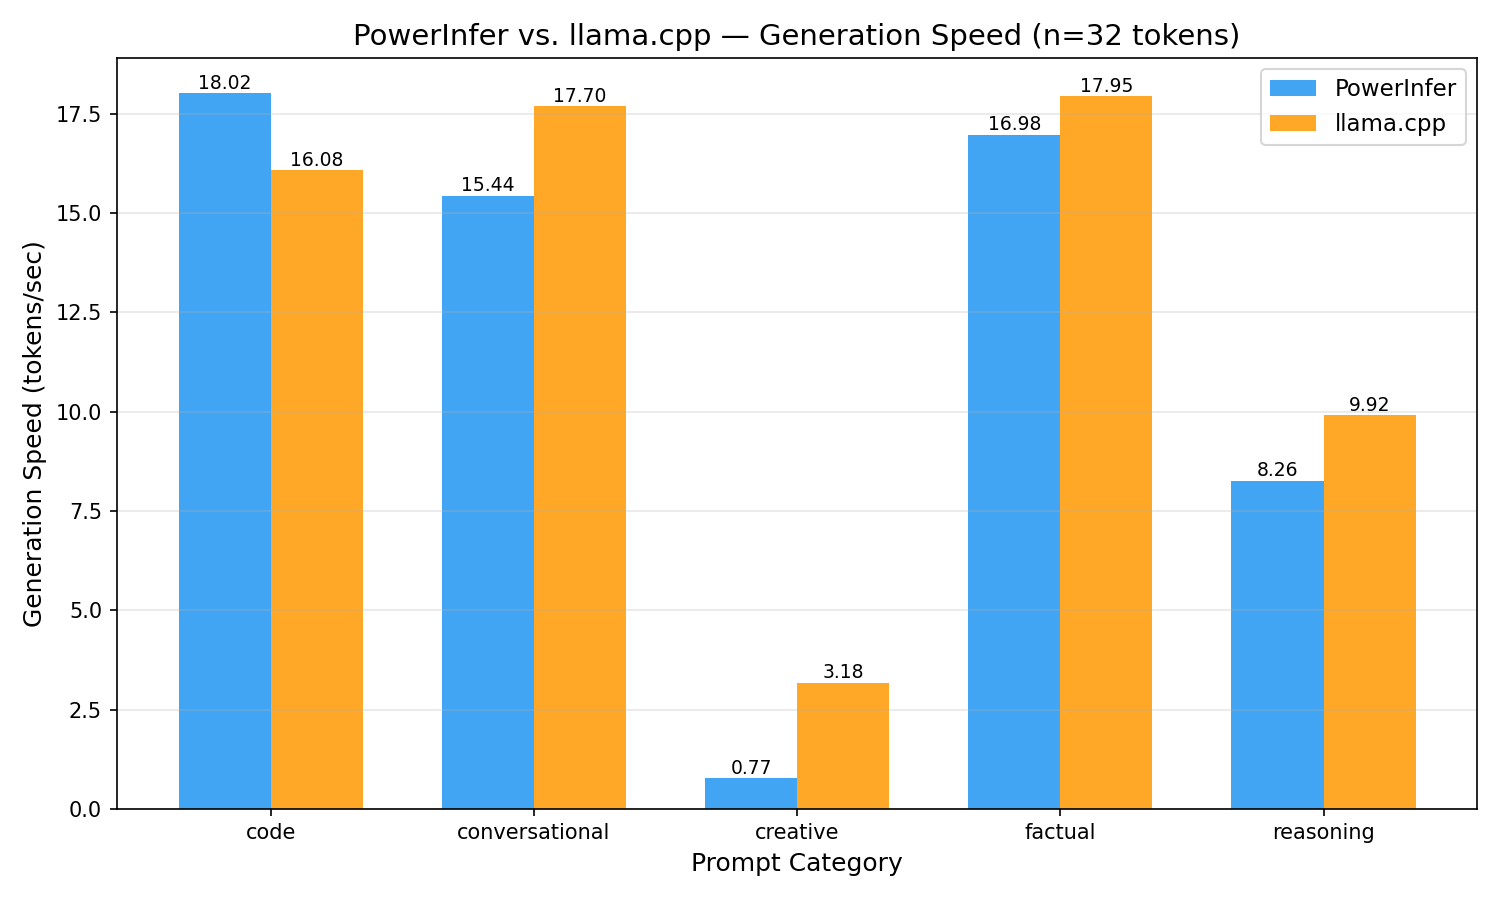
\includegraphics[width=\linewidth]{results/phase3_benchmarks/plot_speed_comparison_n32.png}
    \caption{Apple M4 Max: PowerInfer vs llama.cpp by prompt, $n=32$ tokens.}
    \label{fig:p3-n32}
  \end{subfigure}\hfill
  \begin{subfigure}[t]{0.48\textwidth}
    \centering
    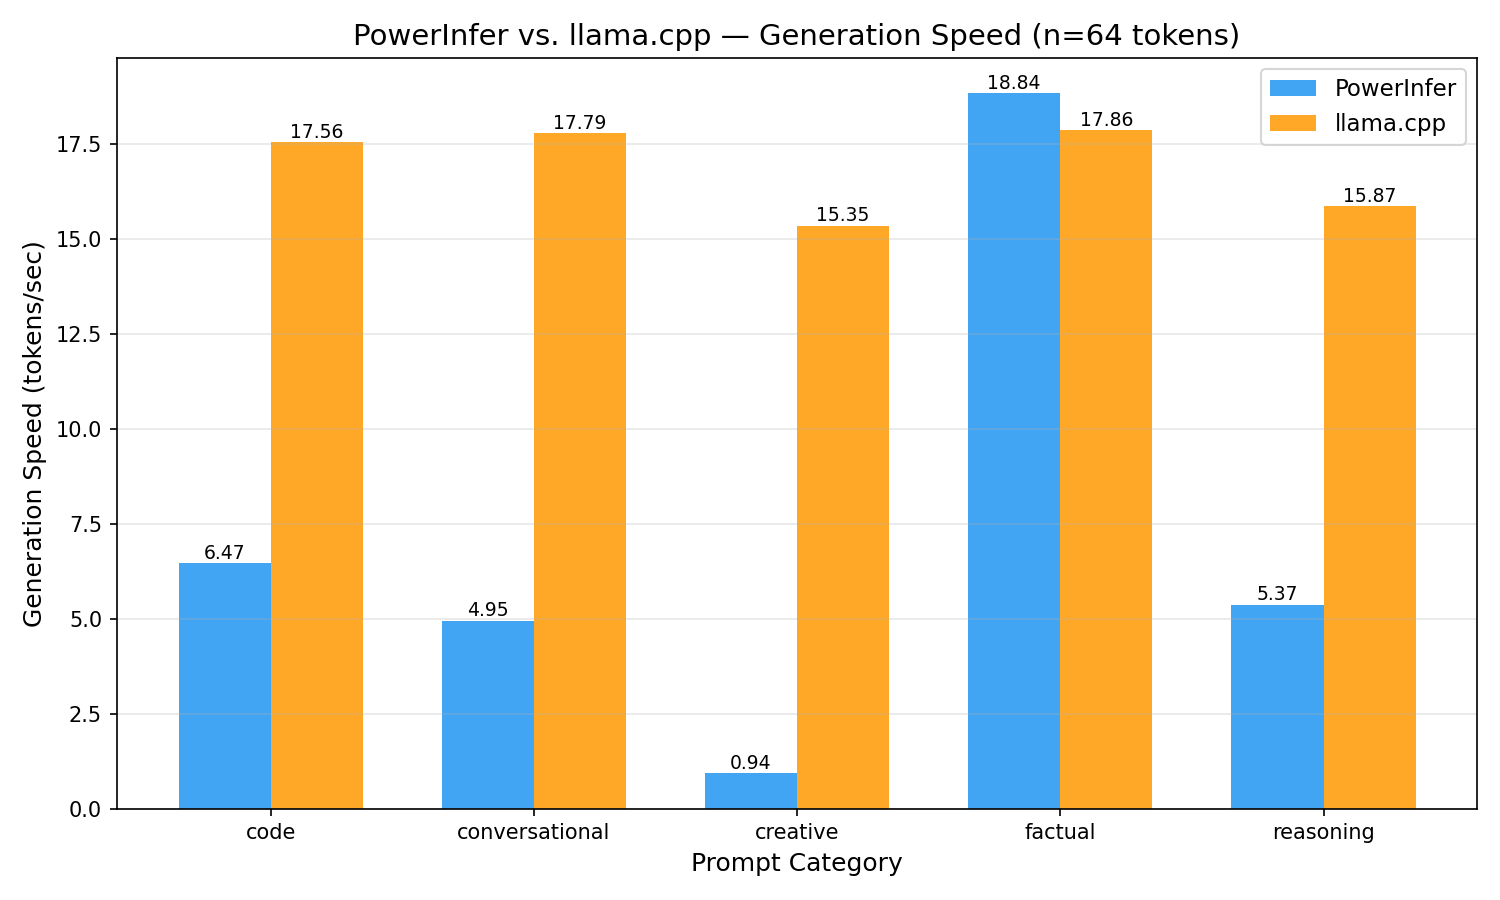
\includegraphics[width=\linewidth]{results/phase3_benchmarks/plot_speed_comparison_n64.png}
    \caption{Same comparison, $n=64$.}
    \label{fig:p3-n64}
  \end{subfigure}
  \par\medskip
  \begin{subfigure}[t]{0.48\textwidth}
    \centering
    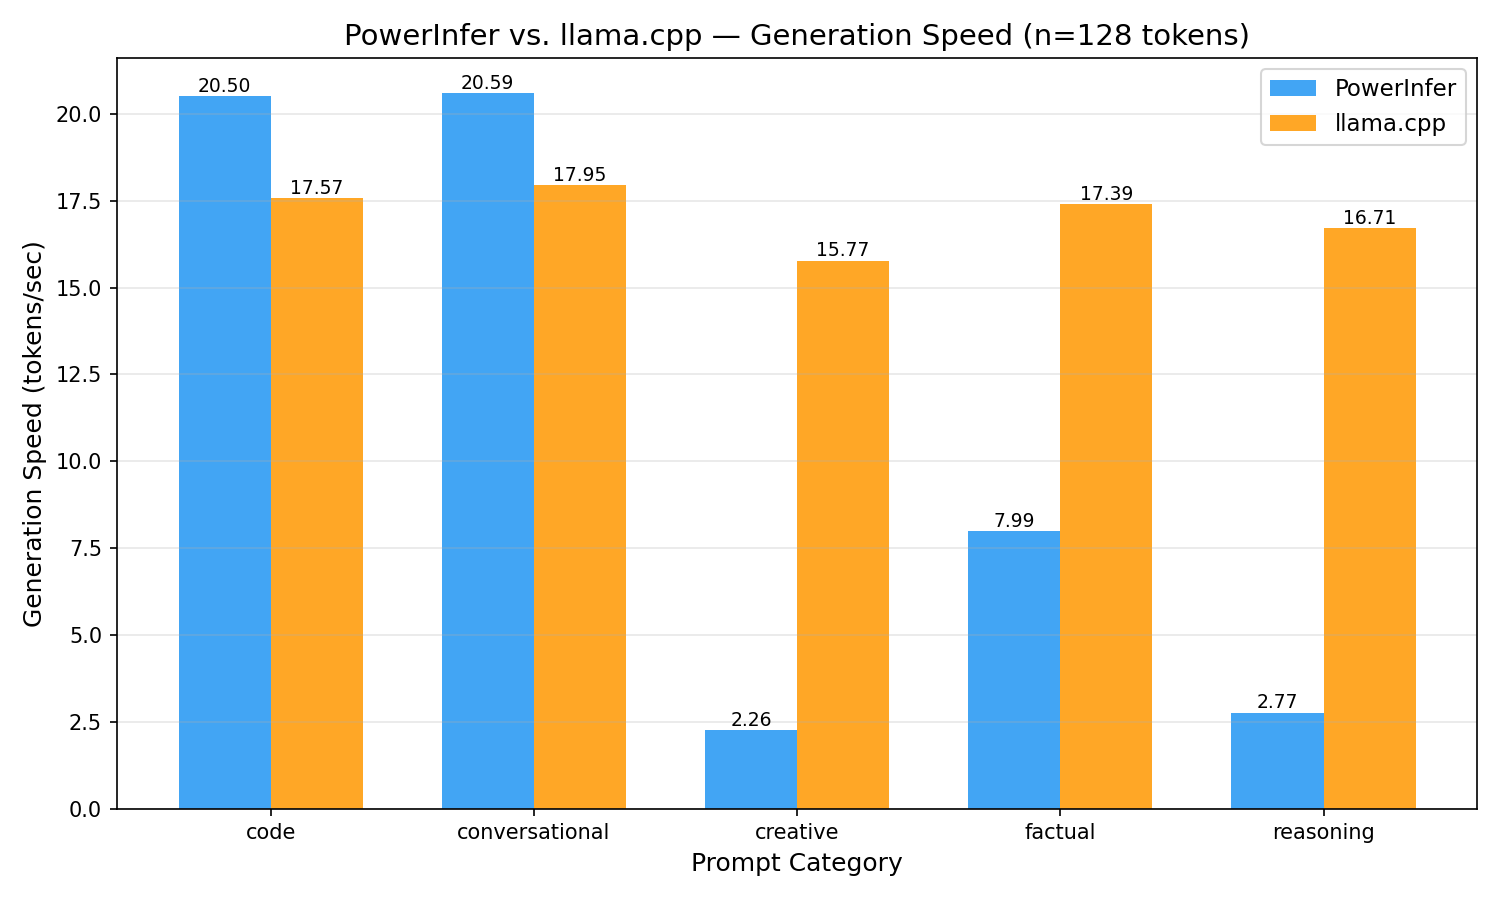
\includegraphics[width=\linewidth]{results/phase3_benchmarks/plot_speed_comparison_n128.png}
    \caption{Same comparison, $n=128$.}
    \label{fig:p3-n128}
  \end{subfigure}\hfill
  \begin{subfigure}[t]{0.48\textwidth}
    \centering
    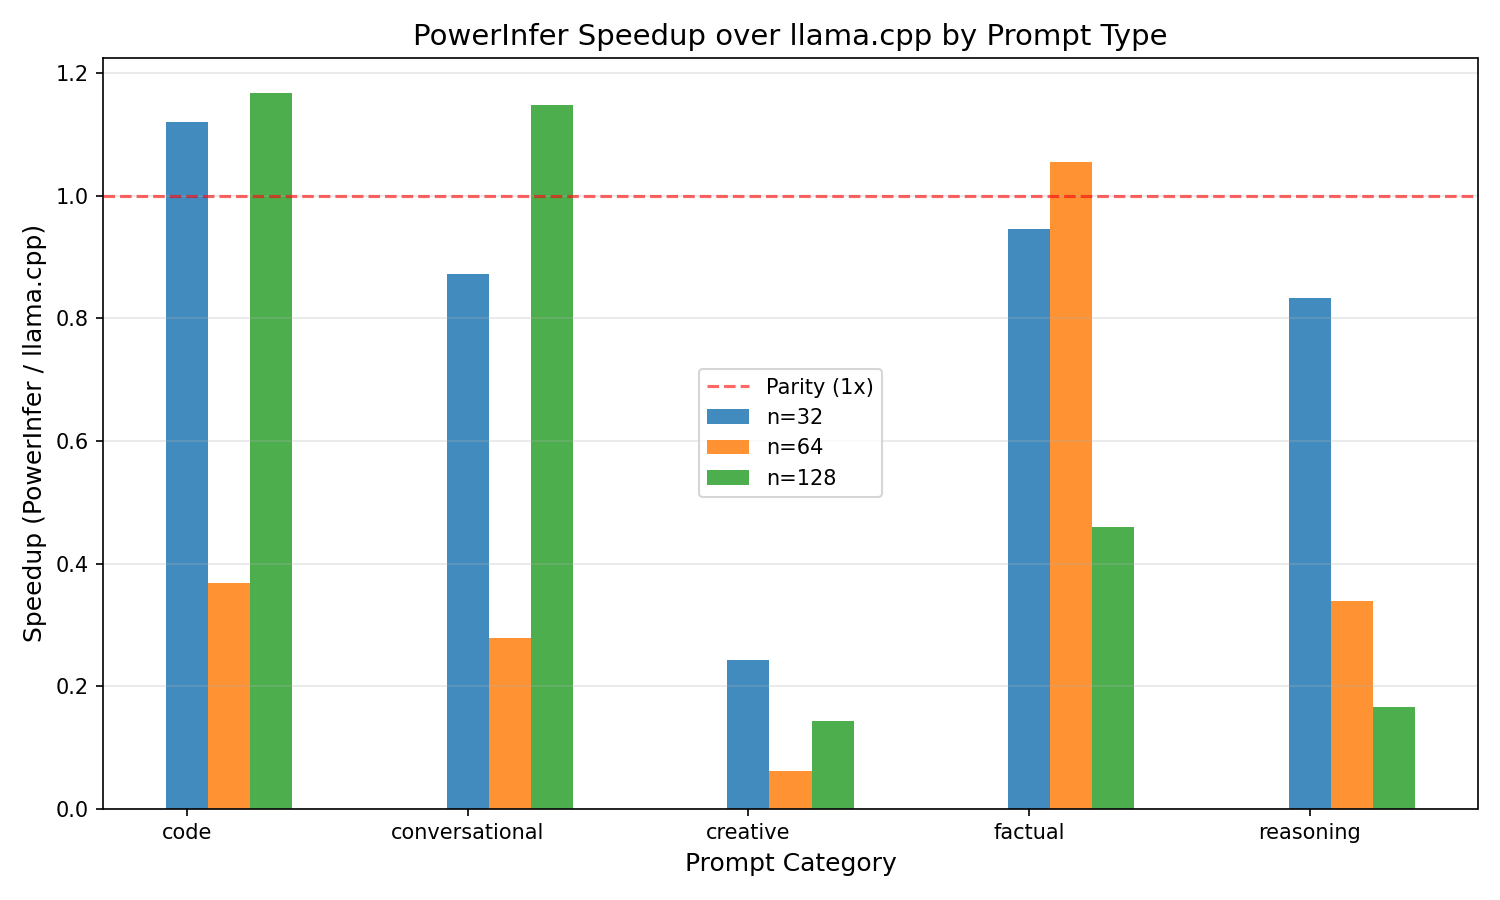
\includegraphics[width=\linewidth]{results/phase3_benchmarks/plot_speedup.png}
    \caption{PowerInfer speedup vs llama.cpp (same runs as (a--c)).}
    \label{fig:p3-speedup}
  \end{subfigure}
  \caption{7B: Apple M4 Max PowerInfer vs llama.cpp---tokens/sec by prompt and relative speedup.}
  \label{fig:p3-7b-cpu}
\end{figure}

\subsection{Phase 4 (7B): cross-prompt hot-neuron overlap}
Average hot-neuron density ranges from \textbf{81.1\% (factual)} to \textbf{85.7\% (reasoning)} of 11008 neurons/layer. Pairwise Jaccard similarity spans \textbf{0.749--0.834} (lowest factual--conversational; highest code--reasoning). Universal hot-neuron counts vary strongly by layer, suggesting static profiling is broadly valid but not perfect.

\begin{figure}[htbp]
  \centering
  \begin{subfigure}[t]{0.48\textwidth}
    \centering
    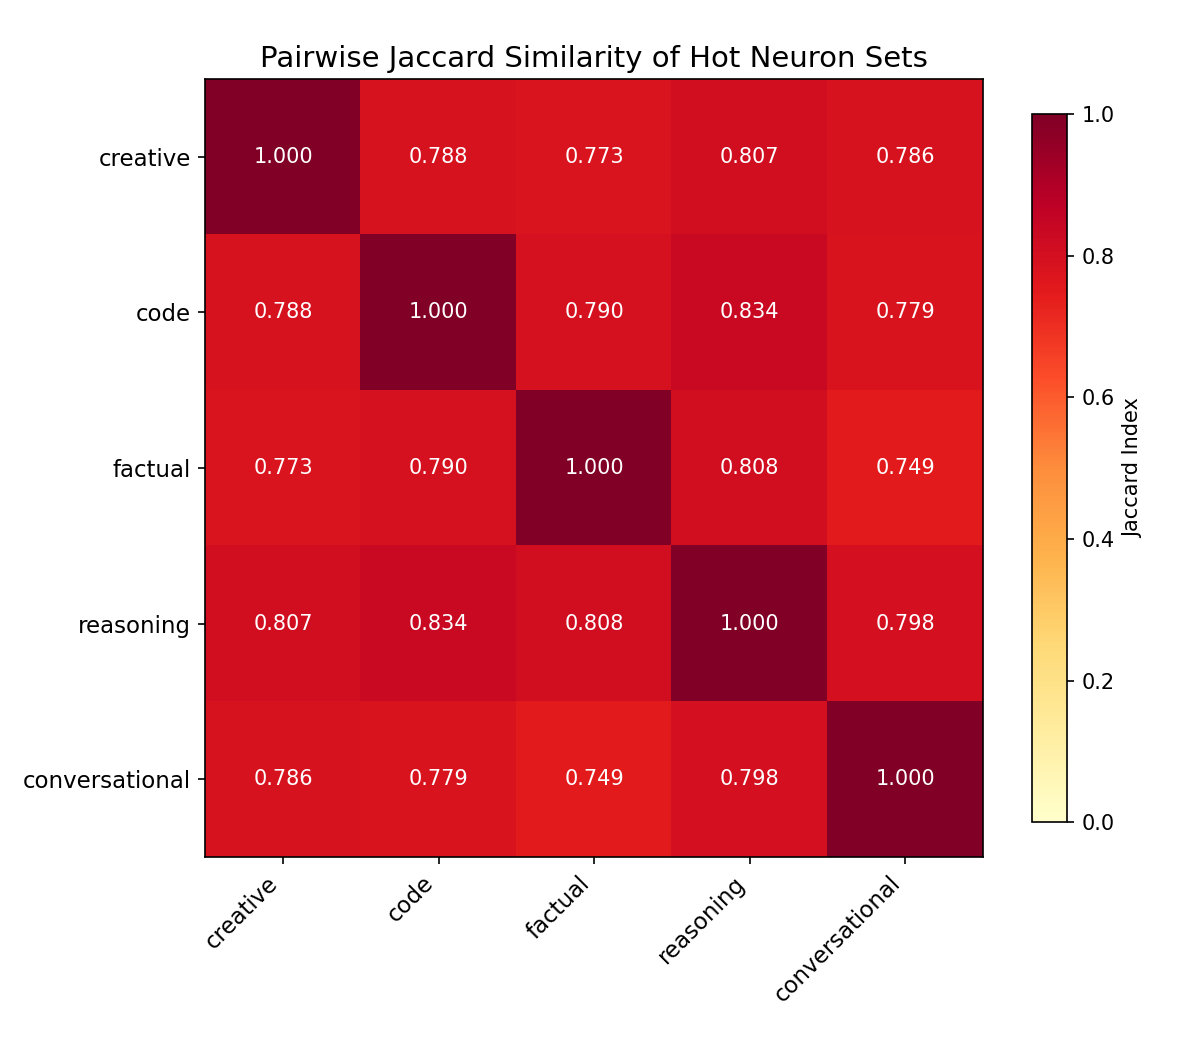
\includegraphics[width=\linewidth]{results/phase4_neuron_variation/plot1_jaccard_heatmap.png}
    \caption{Pairwise Jaccard overlap of hot-neuron sets across the five prompt \textbf{categories} (Phase 4).}
    \label{fig:p4-7b-heat}
  \end{subfigure}\hfill
  \begin{subfigure}[t]{0.48\textwidth}
    \centering
    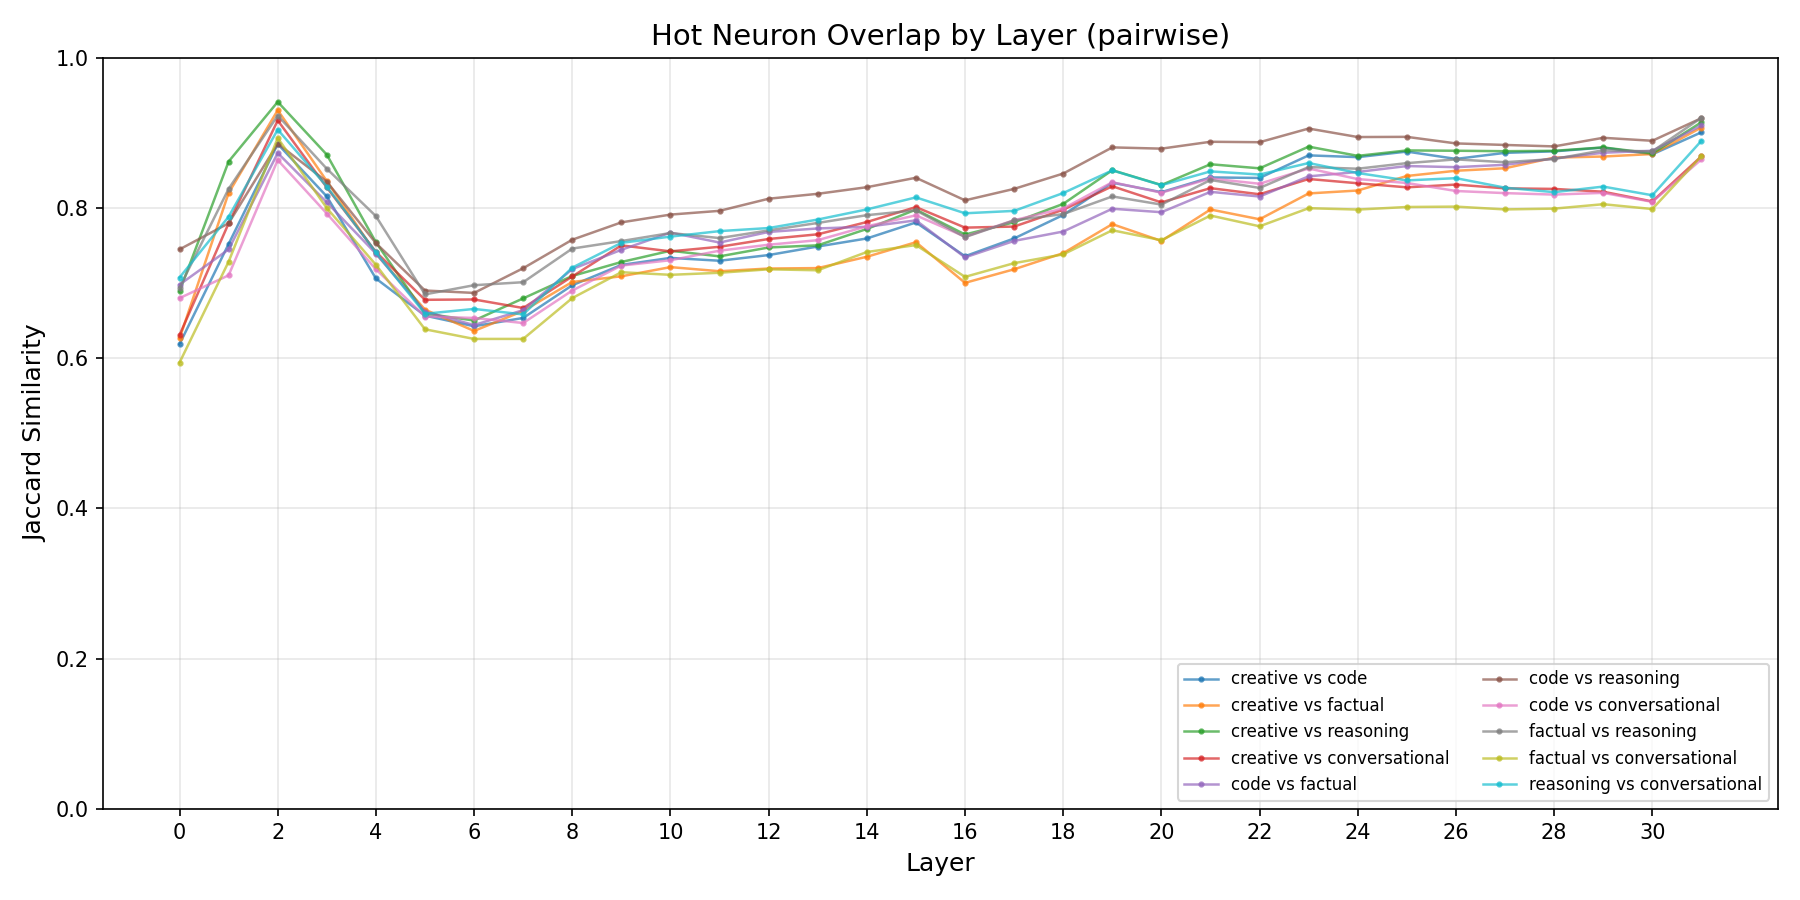
\includegraphics[width=\linewidth]{results/phase4_neuron_variation/plot2_jaccard_by_layer.png}
    \caption{Layer-wise Jaccard for example category pairs (see script defaults).}
    \label{fig:p4-7b-layer}
  \end{subfigure}
  \par\medskip
  \begin{subfigure}[t]{0.48\textwidth}
    \centering
    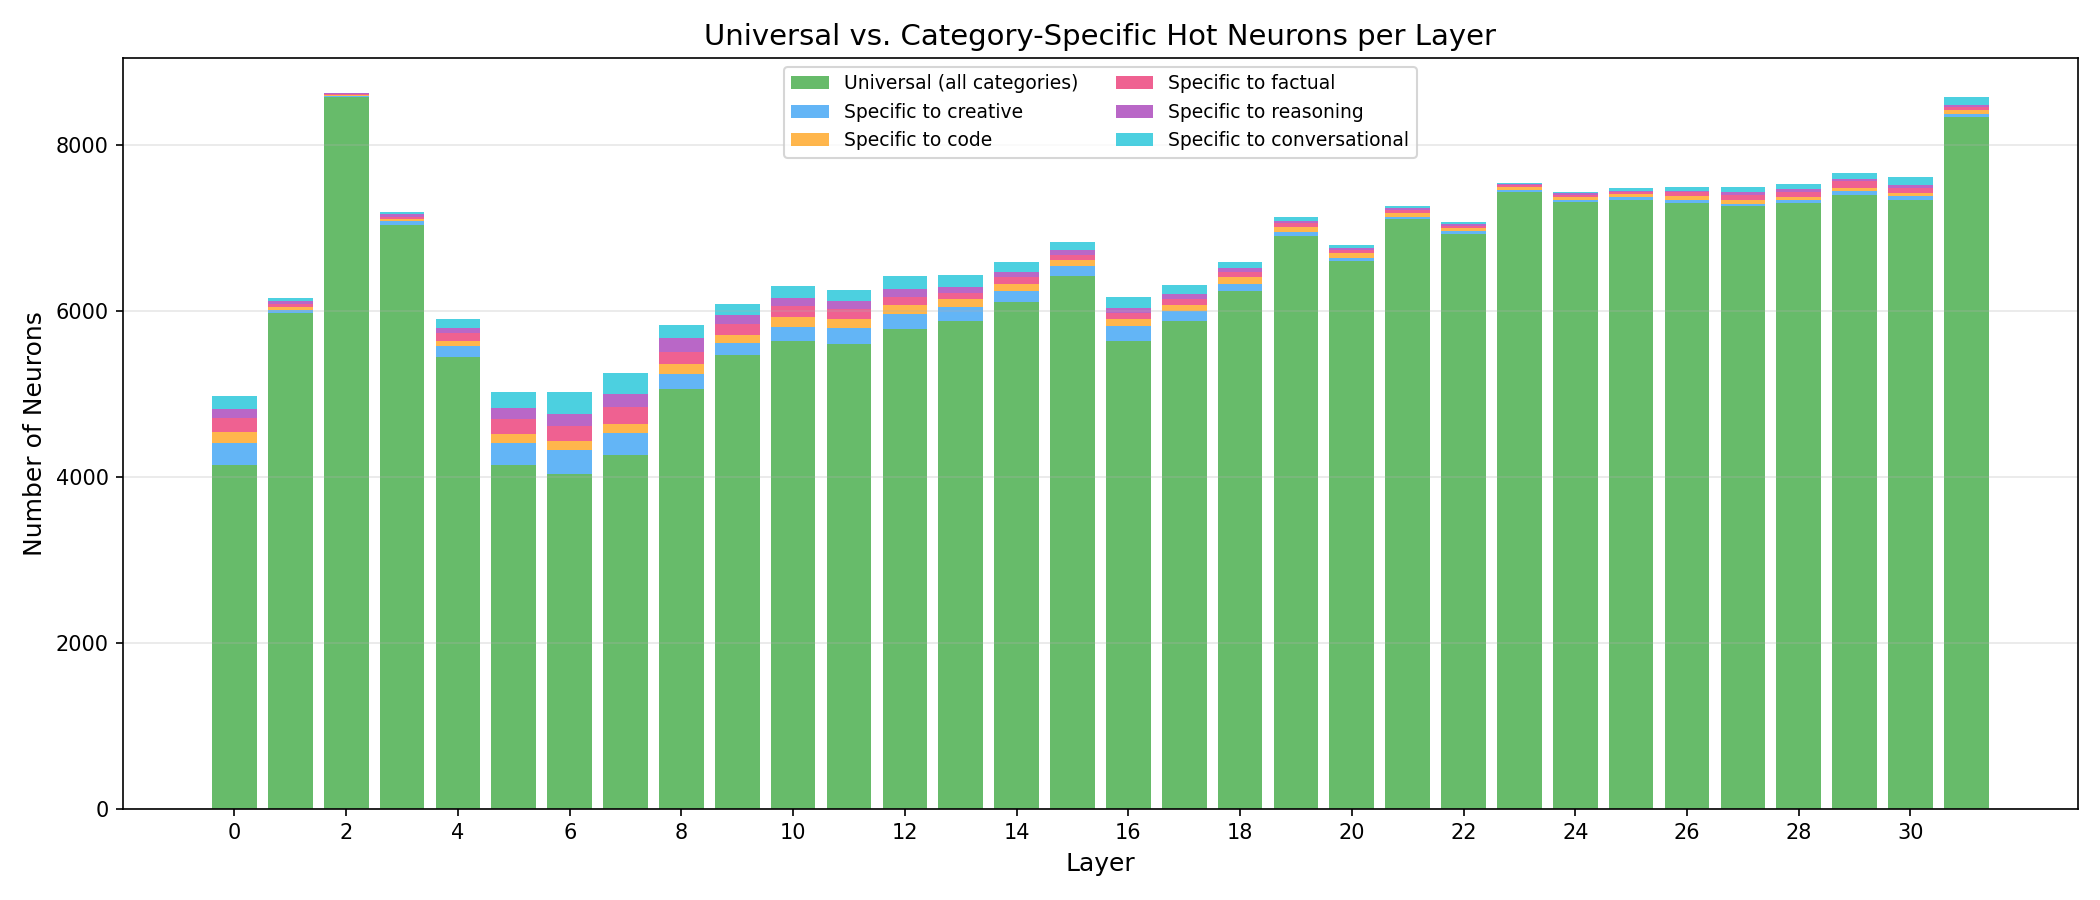
\includegraphics[width=\linewidth]{results/phase4_neuron_variation/plot3_universal_vs_specific.png}
    \caption{Counts of universal vs category-specific ``hot'' neurons by layer.}
    \label{fig:p4-7b-univ}
  \end{subfigure}\hfill
  \begin{subfigure}[t]{0.48\textwidth}
    \centering
    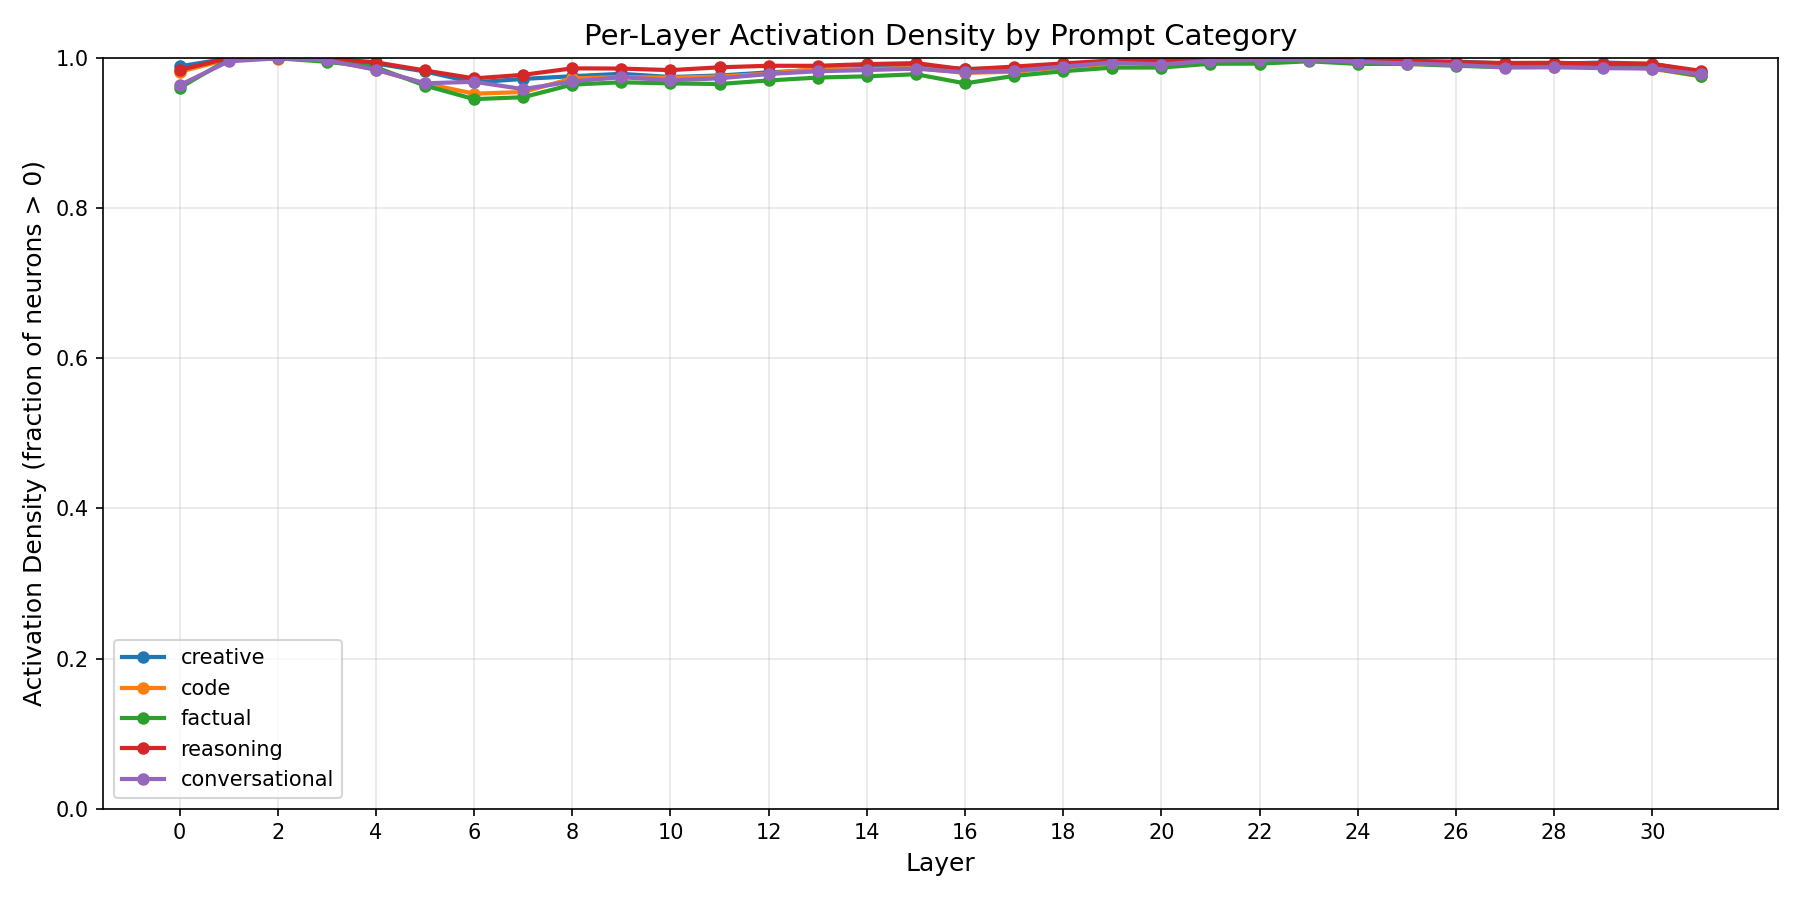
\includegraphics[width=\linewidth]{results/phase4_neuron_variation/plot4_activation_density.png}
    \caption{Per-layer hot-neuron density by prompt category.}
    \label{fig:p4-7b-dens}
  \end{subfigure}
  \caption{7B: cross-prompt hot-neuron overlap and density (ReluLLaMA-7B, Phase~4).}
  \label{fig:p4-7b-grid}
\end{figure}

\subsection{Phase 4 (13B): overlap at larger width}
Hot-neuron density is \textbf{${\sim}73$--$78\%$} of 13824 neurons/layer. Jaccard entries are \textbf{${\sim}0.70$--$0.77$}, slightly lower than 7B, indicating more category-specific mass at wider FFNs while still supporting a substantial shared hot core.

\begin{figure}[htbp]
  \centering
  \begin{subfigure}[t]{0.48\textwidth}
    \centering
    
\includegraphics[width=\linewidth]{results/phase4_neuron_variation_13b/plot1_jaccard_heatmap.png}
    \caption{Category${\times}$category Jaccard (ReluLLaMA-13B hot-neuron overlap).}
    \label{fig:p4-13b-heat}
  \end{subfigure}\hfill
  \begin{subfigure}[t]{0.48\textwidth}
    \centering
    
\includegraphics[width=\linewidth]{results/phase4_neuron_variation_13b/plot2_jaccard_by_layer.png}
    \caption{Layer-wise overlap trends.}
    \label{fig:p4-13b-layer}
  \end{subfigure}
  \caption{13B: cross-prompt hot-neuron overlap (Phase~4, ReluLLaMA-13B).}
  \label{fig:p4-13b-pair}
\end{figure}



\section{Analysis and Discussion}
\textbf{Static profiling vs input diversity.} High Jaccard overlaps support PowerInfer's ``one profile'' design, yet the density spread and layer-wise specialization suggest modest gains from domain-conditioned profiles or layer-aware GPU budgets.

\textbf{Why CPU-only PowerInfer is volatile.} Without GPU residency for hot weights, predictor and indexing overhead can dominate---especially in prefill---making sparse wins inconsistent. This matches PowerInfer's intended deployment: hybrid execution when VRAM is scarce and GPU can hold hot weights.

\textbf{Limitations.} Our vLLM baseline uses SiLU Llama-2, not ReluLLaMA; we do not measure downstream task accuracy; static profiles may drift under domain shift; and tooling assumes single-GPU execution.

\section{Conclusion}
Across ReluLLaMA-7B and 13B we observe consistent \textbf{activation locality} (heavy tails, U-shaped layer-wise skew). Throughput experiments separate dense CPU behavior, dense GPU ceilings, and the intended sparse-hybrid regime: on consumer CPU, PowerInfer can match dense llama.cpp when sparsity aligns but is volatile otherwise; GPU-dense vLLM establishes a higher tok/s ceiling under different activations. Input-type instrumentation shows stable but not identical hot-neuron sets (high Jaccard with structured layer variation), supporting static profiling while motivating lightweight adaptation.

\textbf{Future work:} re-run 13B PowerInfer on Newton with verified offload/build settings; measure quality--speed Pareto; explore layer-aware GPU budgeting informed by universality curves; evaluate domain-conditioned profiles.

\section*{Contribution Statement}
\begin{itemize}
  \item \textbf{Hai Nguyen:} Newton benchmarking (vLLM), report writing (methods/experiments), figure integration.
  \item \textbf{Cuong Dang:} Slide deck development, PowerInfer system explanation, report editing and validation.
  \item \textbf{Joshua Lowe:} Pipeline scripting, reproducibility workflow, llama.cpp baselines and local benchmarking support.
  \item \textbf{Lam Nguyen:} Activation profiling analysis, hot-neuron overlap instrumentation (Phase~4), plots and interpretation.
\end{itemize}

% \input{checklist.tex}
\bibliographystyle{alpha}
\bibliography{references}
\end{document}